\section{Method}
The dataset generation method consists of 3 steps.
First the raw data is gathered form the 3D models.
In the second step, the raw data is masked and cropped to isolate the images of the objects.
In the third step the raw data is combined into randomized ``fake screenshots'', the synthetic training data.
A variety of parameters make it possible to add random variations such as noise, rotations and different objects to the images.
Furthermore, in this step the labels are created by using the dimensions of the masked and cropped object images to automatically generate the labels.
A detailed description of the dataset generation pipeline is shown in Figure \ref{fig:dataset_generation} and will be explained in this chapter.

\begin{figure}[t]
\centering
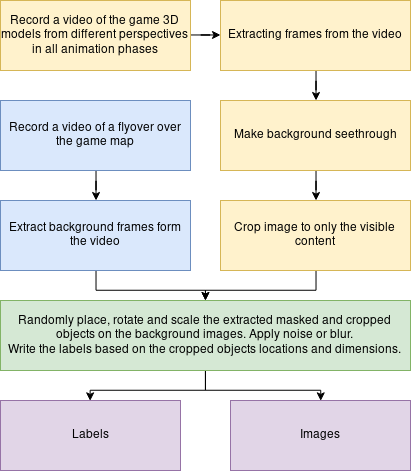
\includegraphics[width=0.4\textwidth]{figures/dataset_generation.png}
\caption{Dataset generation pipeline.}
\label{fig:dataset_generation}
\end{figure}

\subsection{Generating raw data from 3D models}
First the raw data consisting of a set of masked images of the object in each animation phase and from different perspectives is generated.
\subsubsection{Viewing the 3D models}

\begin{figure}[t]
\centering
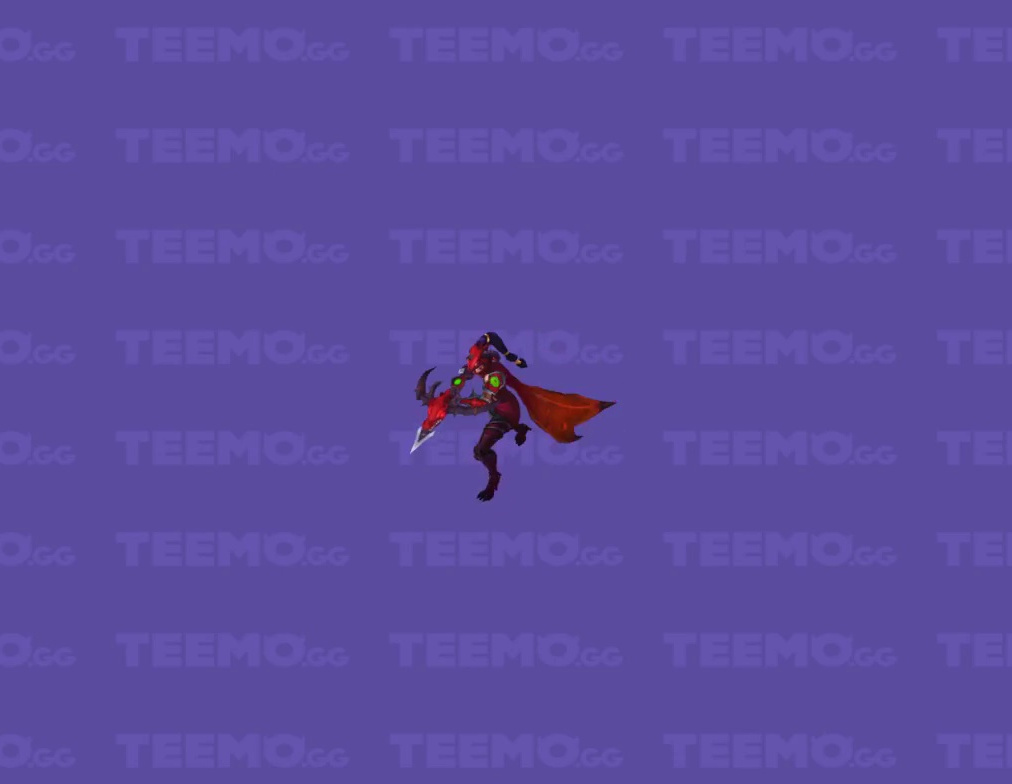
\includegraphics[width=0.4\textwidth]{figures/modelviewer.jpg}
\caption{3D model displayed in the model viewer.}
\label{fig:mv}
\end{figure}

The 3D models of the game characters are extracted and visualized using an online model viewer from \href{https://teemo.gg/model-viewer}{https://teemo.gg/model-viewer}.
The model viewer allows free rotation and zoom around the object as well as playing the characters animations.
Figure \ref{fig:mv} shows a character in the model viewer.
Another model viewer that can be run on a local machine is available on \href{https://github.com/Querijn/LeagueModel}{GitHub}.
\subsubsection{Recording a video and exporting frames}
A video of all animations and all perspectives is then recorded and for the current dataset every third frame is exported using the script \texttt{pyFrameexporter.py}.
Exporting every third frame created about 600-1000 raw object images which is enough to cover all possible animation phases and rotations of the objects.
Figure \ref{fig:mv} shows an exported frame with unicolor background.
The script has the following parameters:
\begin{itemize}
\item \textbf{frames:} Number of frames to skip between each exported frame
\item \textbf{resolution:} Output resolution of each frame
\item \textbf{prefix:} A text prefix to sort the output image files like for example ``output\_{}''.
\end{itemize}

\subsubsection{Masking and cropping the images}
After extracting the images from the videos, the script \texttt{pyExportTransparentPNG.py} is used to remove the uni-color background by modifying the alpha channel of all uni-color pixels.
Afterwards the image is cropped to remaining visible content of the image.
The cropped dimensions of the image will alter be used as the bounding box of the image.
The result of the masking and cropping is shown in Figure \ref{fig:result}.

\begin{figure}[t]
\centering
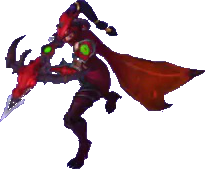
\includegraphics[width=0.2\textwidth]{figures/ultrun_32.png}
\caption{Cropped and masked raw image.}
\label{fig:result}
\end{figure}

The script has the following parameters:
\begin{itemize}
\item \textbf{area:} Area of the input images on which the script is running. The rest of the image will be automatically removed. Especially if the position in the image and size of the object is known defining the area can help accelerate the script.
\item \textbf{background:} The color of the background that shall be transparent in the output image
\item \textbf{tolerance:} The tolerance for each RGB value. Helpful if the background is not exactly the same color everywhere or the outline of the objects in the output is not clean.
\item \textbf{remove\_outline:} Determines how many outline layers of the object should be removed.
Again, if the output objects have artifacts or bad outlines, this can help to remove them.
\end{itemize}

\subsection{Background image raw data}
The game background images are extracted from screenshots of the map recorded in the video game.
Other options would have been to use a high resolution image of the whole map and cut it into pieces.
Also the map is available as 3D model from: \href{https://sketchfab.com/3d-models/for-study-only-summoner-rift-3d-export-ac0a9c6676e34d1ebb184d8e93443c77}{Map 3D model}

\subsection{Other objects}
To further increase the robustness of the synthetic data, I also masked and cropped parts of the game's user interface and cursors.
These objects are placed on the screenshots as well to make the object detector learn what happens when a cursor is overlapping an objects and to not detect things on the UI.

\subsection{Generating synthetic training data}
With the raw data split in their categories (structures, minions, player characters), we can now generate synthetic game images.
Algorithm \ref{alg:1} and \ref{alg:2} describe the process.

\begin{algorithm}
\hspace*{\algorithmicindent} \textbf{Input:} dataset\_size, raw\_background, raw\_objects, num\_objects, max\_rotation, max\_scale\\
\hspace*{\algorithmicindent} \textbf{Output:} image, label
\begin{algorithmic}[1]
\caption{Generation of a synthetic labeled image}
\label{alg:1}
\Function{generate\_dataset}{}
\For{dataset\_size}
\State \textit{N} $\gets$ random([0,num\_objects])
\State cur\_image $\gets$ random(raw\_background))
	\For{\textit{N}}
	\State cur\_object $\gets$ random(raw\_objects)
	\State position $\gets$ random(cur\_image)
	\State scale $\gets$ random([-max\_scale, max\_scale])
	\State rotation $\gets$ random([-max\_rotation, max\_rotation])
	\State \texttt{add\_object(cur\_image, cur\_object, rotation, scale, object\_class, position)}
	\EndFor
\State \texttt{apply\_noise()}
\State \texttt{apply\_blur()}
\EndFor
\EndFunction
\end{algorithmic}
\end{algorithm}

\begin{algorithm}
\hspace*{\algorithmicindent} \textbf{Input:} cur\_image, raw\_object, rotation, scale, object\_class, position
\\
\hspace*{\algorithmicindent} \textbf{Output:} image, label
\begin{algorithmic}[1]
\caption{Add an object to an image}
\label{alg:2}
\Function{add\_object}{}
\State \texttt{scale\_object(scale)}
\State \texttt{rotate\_object(roation)}
\For{\textbf{all} cur\_pixels \textbf{in} cur\_image}
	\If {cur\_pixel is covered by object}
	\State cur\_pixel $\gets$ object\_pixel
	\Else
	\State cur\_pixel $\gets$ cur\_pixel
	\EndIf
\EndFor
\State \texttt{append\_to\_labels(obejct\_class, object\_center, width, height)}
\EndFunction
\end{algorithmic}
\end{algorithm}

\begin{figure*}[t]
\centering
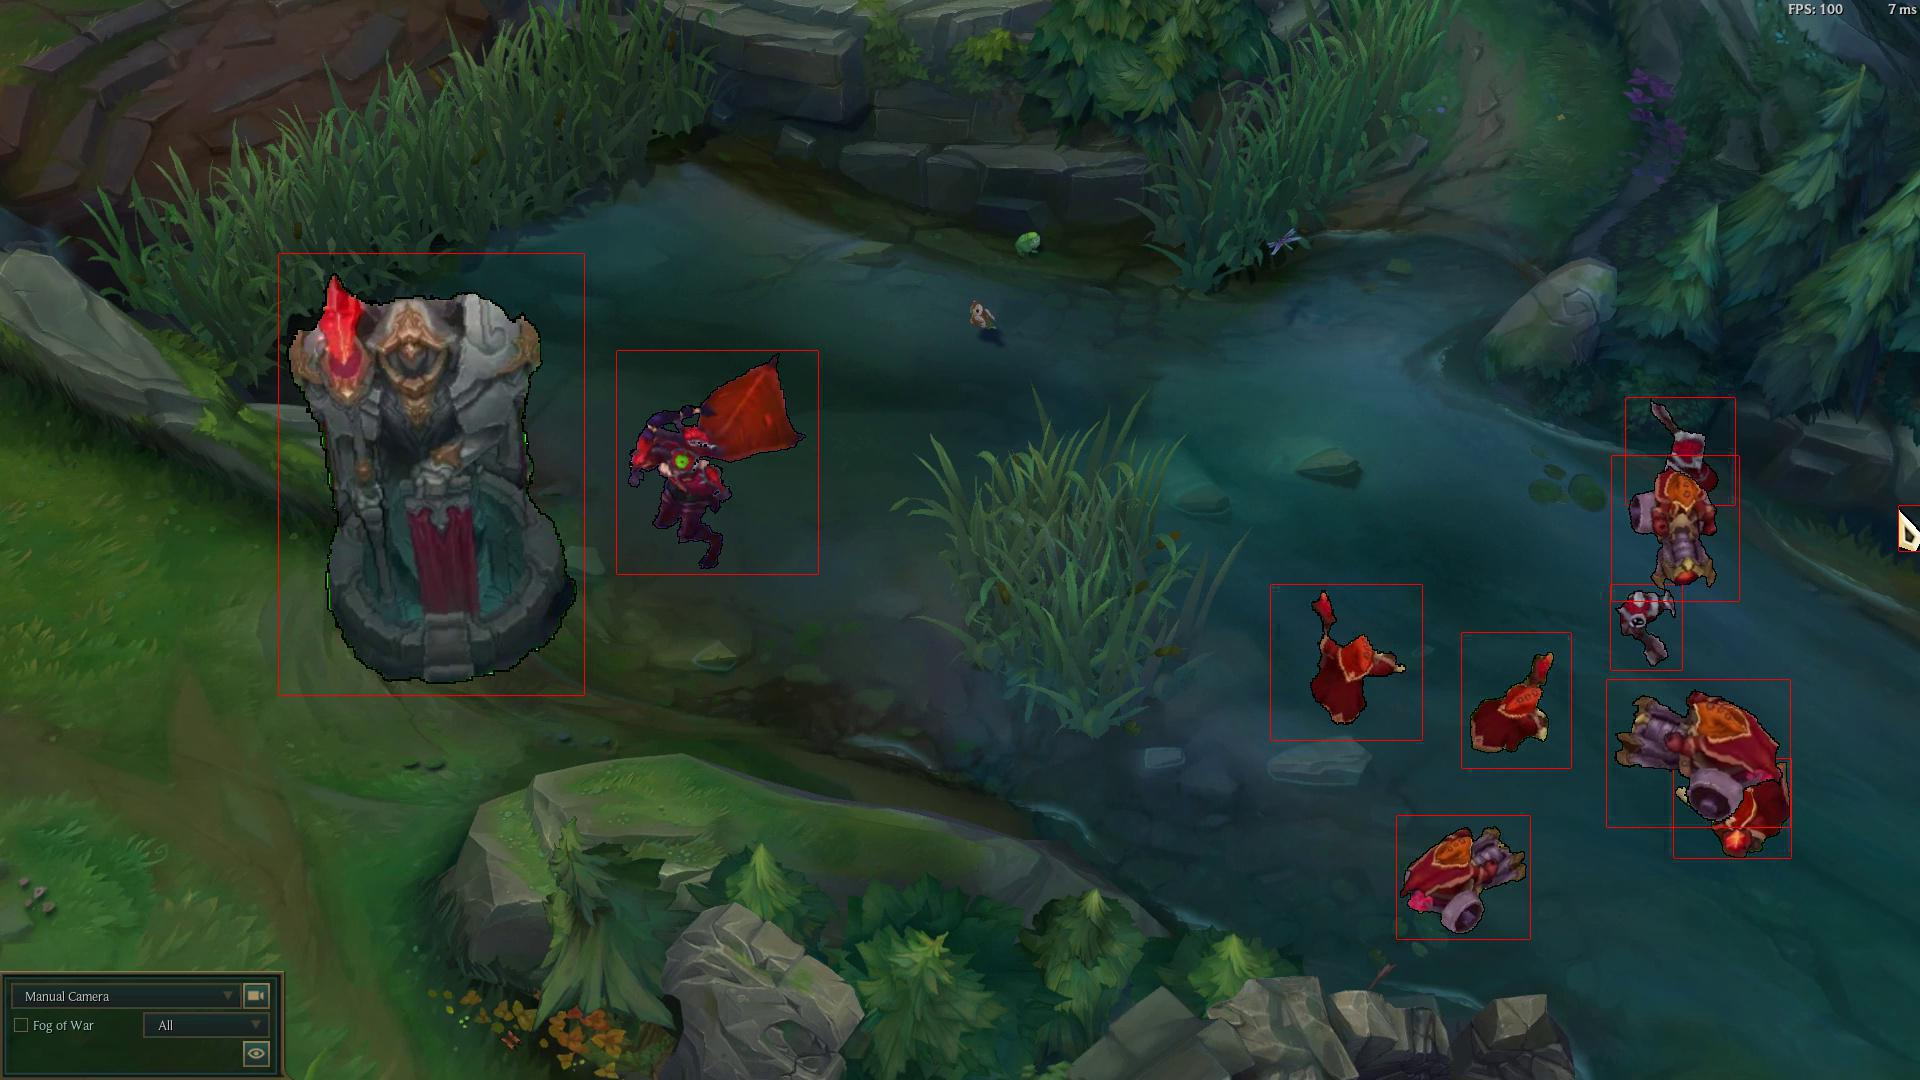
\includegraphics[width=0.8\textwidth]{figures/example.jpg}
\caption{An automatically generated labeled image. The red boxes visualize the generated label. Note how the minions are overlapping and clustered around the bias point to simulate their behavior of clumping up during fighting.}
\label{fig:example}
\end{figure*}

Figure \ref{fig:example} shows an artificially generated labeled data. For the sake of visualization no noise or blur have been applied. 

In the following sections different variations and parameters of the algorithm are explained.
Note that each of the additional ways of modifying the images can be turned off individually.

\subsubsection{Placement}
In this step the raw data is placed on a randomly selected background image.
The placement of the objects is important to generate realistic game screenshots and to make the object detector more robust.
During the game, the objects will overlap.
On top of the game the cursor and the user interface will overlap the game.
To reproduce this layering, the following parameters allow to modify the way in which the objects are placed.
\begin{itemize}
\item \textbf{cursor\_max/min, champion\_max/min, minion\_max/min, tower\_max/min}: Set the minimum/maximum number to control how often objects are placed. A number of objects between the min and max value will be uniformly picked.
\item \textbf{overlay\_chance}: Probability of adding UI elements to the image 
\item \textbf{fog\_of\_war}: Probability to add fog of war to the image
\end{itemize}

The position at which an object is placed is chosen randomly by uniformly selecting a \textit{x} and \textit{y} coordinate in the image.

\paragraph*{\textbf{Grouping minions}}
In the real game groups of computer controlled minions will usually fight each other and thus usually group up and overlap more often.
To simulate this effect, the minions are not only placed randomly on the image, but can be placed around a bias point using a normal distribution.
The parameter \textbf{bias\_strength} can be used to adjust the way the minions are clustered.

\subsubsection{Scale and rotate}
Parameters allow to set the input scale and orientation of each object in the image.
Additionally, the parameters \textit{max\_scale} and \textit{max\_rotation} set the maximum amount of the random scaling and rotation applied to the input values.ö
Choosing scale and rotation for an object is picking a rotation and scale value between the given maximum values and add/subtract it from the input orientation and scale.
The parameter \textbf{sampling\_method} can be used to chose different sampling methods for scaling the image.
Since the results of different sampling methods can look different, this can further improve the robustness of the dataset.

\subsubsection{Noise and blur}
To make the dataset more robust to in game effects like particles covering or coloring the characters, noise is introduced.
Random noise is applied by randomly chaning the RGB values of the final image.
The parameter \textbf{noise} can be used to adjust the strength of the noise for each individual channel.
Gaussian blur is applied to smoothen the image.
The parameter \textbf{blur\_strength} is used to set the strength of the blur.

\subsubsection{User Interface}
During testing the user interface of the real game was not included in the training data and thus led to significant wrong detections.
Therefore, I created masked versions of the game UI and replace champion specific icons with a random selection of icons.
Another problem was the quite frequently occurring overlapping of the player's mouse cursor especially with minions (in order to attack them for example).
To solve this I created raw images of the cursor graphics which are added in random locations on the image.